\documentclass{article}
\usepackage{josuamathheader}
\begin{document}

\section*{Aufgabe 3}
\begin{enumerate}
    \item 
    Aus $x' = y' = 0$ folgt sofort $x= 0$ und dann auch $y = 0$, d.h. $y* = (0,0)$ ist der Gleichgewichtspunkt des Systems.
    Das linearisierte System ist dann gegeben durch 
\[ 
    \begin{cases}
        x'&= x\\
        y'&= -y
    \end{cases} \Leftrightarrow \begin{pmatrix}
    x'\\y'
\end{pmatrix} = \begin{pmatrix}
    1 & 0\\0 &-1
\end{pmatrix} \begin{pmatrix}
    x\\y
\end{pmatrix}.
\]
Die Eigenwerte sind offensichtlich gegeben durch $1$ und $-1$ und wir können die Eigenräume direkt ablesen:
\[
    E_{1}(A) = E^-(A) = \operatorname{Span}  \begin{pmatrix}
    1\\0
\end{pmatrix}, \qquad E_{-1}(A) = E^+(A) = \operatorname{Span} \begin{pmatrix}
    0\\1
\end{pmatrix}
\]
\begin{center}
    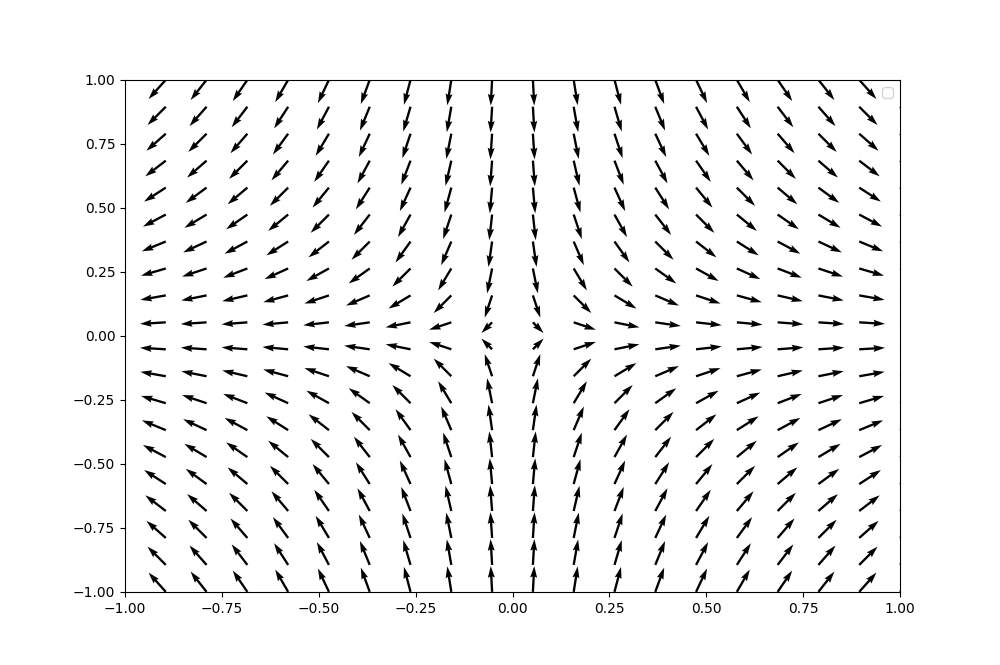
\includegraphics[width = \textwidth]{figure_07_1.png}
\end{center}
\item $y^*$ ist in beiden Eigenräumen enthalten und damit ein Sattelpunkt im linearen System.
Zum linearisierten System gehört der Fluss
\[
    \Phi_t^\mathrm{l}\begin{pmatrix}
        x_0\\y_0
    \end{pmatrix} = \begin{pmatrix}
        x_0e^t\\y_0e^{-t}
    \end{pmatrix}.
\]
Das nichtlinearisierte System ist gegeben durch
\[
    \begin{pmatrix}
        x'\\y'
    \end{pmatrix} = \begin{pmatrix}
        1&0\\0&-1
    \end{pmatrix} \begin{pmatrix}
        x\\y
    \end{pmatrix} + 4x^3 = A\cdot \begin{pmatrix}
        x\\y
    \end{pmatrix} + g\begin{pmatrix}
        x\\y
    \end{pmatrix},
\]
wobei $g$ differenzierbar mit $g'\begin{pmatrix}
    x\\y
\end{pmatrix} = 12x^2$ und daher auf einer Umgebung $U$ stets eine beschränkte Ableitung besitzt.
Der zugehörige Fluss ist gegeben durch
\[
    \Phi_t^\mathrm{nl}\begin{pmatrix}
        x_0\\y_0
    \end{pmatrix} = \begin{pmatrix}
        x_0e^t\\ (x_0)^3e^{3t} + (y_0 - x_0^3)e^{-t}
    \end{pmatrix},
\]
denn:\\
Die Differentialgleichung in der ersten Komponente ist unabhängig von der zweiten Komponente und ist bekanntlich eindeutig lösbar durch $x = x_0e^t$.
In der zweiten Komponente folgt die Eindeutigkeit aus dem Satz von Picard-Lindelöf, da $-y + 4(x_0^3e^{3t})$ lokal Lipschitz-stetig in $y$ ist.
Es gilt 
\[
    y' = 3x_0^3e^{3t} - (y_0 - x_0^3)e^{-t} = -x_0^3e^{3t} - (y_0-x_0^3)e^{-t} + 4(x_0e^t)^3 = -y + 4x^3
\]
und
\[
    y(0) = x_0^3 + (y_0 - x_0^3) = y_0.
\]
Insbesondere ist also $y$ eine Lösung des Anfangswertproblems. Diese ist nach Picard-Lindelöf aber eindeutig.

Insgesamt ist also Satz 3.18 anwendbar und es folgt, dass
$\Phi_t^\mathrm{nl}$ und
\[
    e^{tA} \overset{A \text{ diagonal}}{=} \begin{pmatrix}
        e^t & 0\\0&e^{-t}
    \end{pmatrix} = \Phi_t^\mathrm{l}
\]
topologisch konjugiert sind.
$y^*$ ist in beiden Systemen der Fixpunkt, d.h. die beiden Punkte werden aufeinander abgebildet unter der topologischen Konjugation.
Insbesondere ist also $y^*$ auch im nichtlinearisierten System ein Sattelpunkt.
Sei $(x_0, y_0)$ ein Element der stabilen Menge.
Dann muss gelten $\lim\limits_{t \to \infty} x_0e^t = c \in \R \implies x_0 = 0$.
Weiter muss gelten $\lim\limits_{t \to \infty} x_0^3e^{3t} + (y_0 - x_0^3)e^{-t} = \lim\limits_{t \to \infty} y_0e^{-t} = 0$ für beliebiges $y_0$. Die stabile Menge ist also gegeben durch $\operatorname{span}\begin{pmatrix}
    0\\1
\end{pmatrix}$ im Vektorraum $\R^2$.
Sei nun $(x_0, y_0)$ Element der instabilen Menge.
Dann gilt für beliebiges $x_0$ $\lim\limits_{t \to -\infty} x_0e^t = 0$. Weiter muss gelten
$\lim\limits_{t \to -\infty} (x_0)^3e^{3t} + (y_0 - x_0^3)e^{-t} = (y_0 - x_0^3) \lim\limits_{t \to -\infty}  e^{-t}$.
$\lim\limits_{x \to \infty} e^{-t}$ divergiert, also muss $y_0 = x_0^3$ gelten.
Wir erhalten als instabile Menge die Menge aller $(x_0, x_0^3)$ für $x_0 \in \R$.
\item Betrachte die Abbildung
\[
    \Psi\colon \begin{pmatrix}
        a\\b
    \end{pmatrix} \mapsto \begin{pmatrix}
        a\\b - a^3
    \end{pmatrix}.
\]
Dann gilt für beliebige $x_0, y_0 \in \R$
\begin{align*}
    \Phi_t^\mathrm{l} \circ \Psi \begin{pmatrix}
        x_0 \\y_0
    \end{pmatrix} &= \Phi_t^\mathrm{l} \begin{pmatrix}
        x_0\\y_0-x_0^3
    \end{pmatrix}\\
    &= \begin{pmatrix}
        x_0e^t\\
        (y_0 - x_0^3)e^{-t}
    \end{pmatrix}\\
    &= \begin{pmatrix}
        x_0e^t\\
        x_0^3e^{3t} + (y_0 - x_0^3) - (x_0e^t)^3
    \end{pmatrix}\\
    &= \Psi \begin{pmatrix}
        x_0e^t\\
        x_0^3e^{3t} + (y_0 - x_0^3)e^{-t}
    \end{pmatrix}\\
    &= \Psi \circ \Phi_t^\mathrm{nl} \begin{pmatrix}
        x_0\\y_0
    \end{pmatrix}.
\end{align*}
\item Phasendiagramm des nichtlinearisierten Systems: \begin{center}
    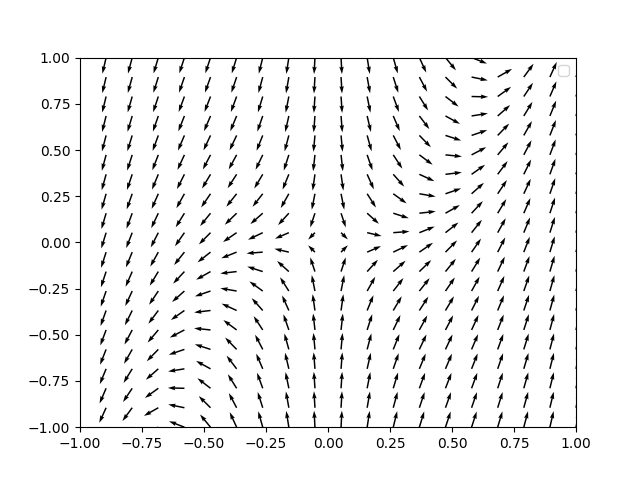
\includegraphics{figure_07_2.png}
\end{center}
\end{enumerate}
\end{document}